\chapter{Konfiguration}\label{cha:configuration}
\xc ist ein hoch konfigurierbares Segelflugrechnerprogramm und kann sehr flexibel auf die jeweiligen Vorlieben
und Bedürfnisse angepasst werden.

Dies Kapitel beschreibt die Konfigurationsmöglichkeiten und  -optionen.
\section{Übersicht der Konfiguration}\index{Konfiguration}
Mögliche  Änderungen der Konfigurationsvoreinstellungen innerhalb \xc, welche hier behandelt werden:
\begin{itemize}
\item Ändern von  Konfigurationseinstellungen. Dies ist die Art von Konfiguration, die die meisten
    Benutzer anwenden werden, da die internen Konfigurationen teilweise genauere Kenntnis benötigen.
    Mithilfe dieser Möglichkeiten können so gut wie alle notwendigen  Einstellungen vorgenommen werden.
    Das Hauptaugenmerk in diesem Kapitel beschäftigt sich daher mit diesen Konfigurationsvoreinstellungen.
 \item Ändern der Benutzersprache, oder wenigstens ändern der Texte innerhalb der
     Informationsfenster.
\item Ändern der Zuordnung von Buttons und Menüs. Es können Inhalt und Struktur der Buttonmenüs
    geändert werden.
\item Ändern oder Zuordnen von Aktionen, welche stattfinden sollen, wenn bestimmte Ereignisse
    auftreten.
\item Definieren, wie lange Statusmeldungen erscheinen und/oder welcher Sound dazu gespielt werden
    soll.
\end{itemize}
Da es sich bei \xc  um ein quelloffenes OpenSource System handelt, ist die Beschreibung aller
Möglichkeiten der Einstellungen in diesem Kapitel so gut wie unmöglich. Prinzipiell kannst Du \xc auch
selber kompilieren und wirklich \textbf{alles} ändern.

Solltest Du ein ernstes Interesse daran haben, wirklich detailliert in \xc  einzusteigen, um eventuell Deine
ganz eigene Oberfläche zu gestalten, so empfehlen wir,  Dich mit dem \xc-Wiki  zu beschäftigen. Hier der
Link: \url{http://www.xcsoar.org/trac/wiki}


%%%%%%%%%%%%%%%%%%
\section{Ändern der Voreinstellungen}
Es gibt einen Menge an Einstellungen, welche vom Benutzer verändert werden
können. Bis auf das generelle Layout des Programmes kann
\menulabel{\bmenut{Konfig.}{2/3}\blink\bmenut{System}{Einstellung}} sogut wie alles verändert und
an eigene Vorlieben angepasst werden.

Du solltest es tunlichst unterlassen, an diesen Einstellungen während des Fluges
''herumzufummeln'', hier sollte Deine Aufmerksamkeit voll und ganz dem Fluge und
Deiner Umgebung gewidmet sein. \warning

Alle Einstellungen sollten bereits vorher am Boden erfolgt sein, so daß derartige
Änderungen in der Luft nicht mehr notwendig sind.

Die Konfiguration wird über zwei Ebenen aufgerufen, in denen weitere Fenster aufgerufen werden können.
Die Dialoge zum Ändern  der Voreinstellungen sind dann auf mehrere Seiten verteilt.

\begin{center}
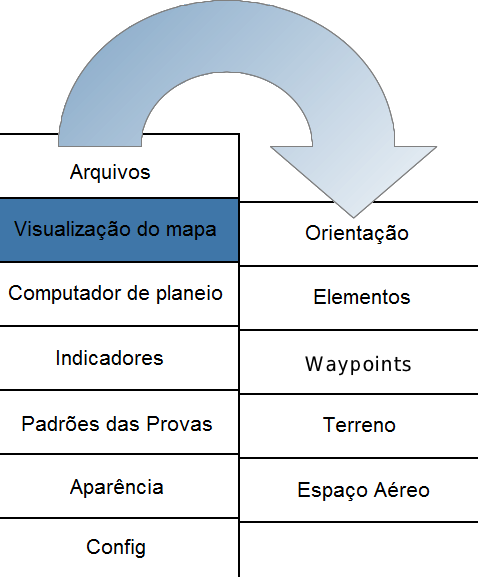
\includegraphics[angle=0,width=0.5\linewidth,keepaspectratio='true']{figures/config-menu.png}
\end{center}

Wenn Du eine Änderung vorgenommen hast und diese speichern willst, drücke auf \button{Schließen} oder
den Power-Knopf des \al .

Ein weiterer Tastendruck bringt Dich zurück auf die normale Kartenoberfläche.

\tip Wenn alles zu Deiner Zufriedenheit eingestellt wurde, ist es angeraten, ein eigenes Profil
abzusichern, um diese Einstellungen jederzeit problemlos restaurieren zu können. Damit können u.a. auch
andere Flieger Ihre eigenen, ganz speziellen Vorliegen für einen Schnellzugriff abspeichern.
Auch, falls dem PDA mal  die Batterie ausgeht, ist zur schnellen Wiederherstellung der persöhnlichen
Einstellungen wenigestens das Sichern eines solchen Files eine große Hilfe.

Falls ein oder mehrerer Konfigurationsfiles \verb''xcsoar-registry.prf''  bestehen, so wird beim Start als allererstes nach
einem dieser Files zur Auswahl gefragt.

Im Kap.~\ref{cha:data-files} werden die diversen Formate dieser Files mit ihren
Auswirkungen auf das System besprochen.

Um die Suche bzw. Auswahl und Übersicht einfacher zu machen, bleibt,
wenn kein File benutzt bzw. angelegt werden muß, bleibt das Auswahlfeld einfach leer.

Das Hauptkonfigurationsfenster (System-Einstellung) kann im ''Basis'' oder
''Experten''-Modus durch Anklicken eines Häkchen ''Experte'' bearbeitet werden.
\sketch{figures/config-expert.png}\index{Experten-Modus}\index{Basis-Modus}

''Basis''-Modus sind einige der weniger für die Funktion wichtigen Parameter für den
einfacheren Überblick verborgen. 

\tip In der folgenden Beschreibung werden alle die
Parameter, die nur im Expertenmodus sicht- und auswählbar sind, mit
einem$^{\textcolor{blue}{\star}}$ versehen.


%%%%%%%%%%%%%%%%%%
\section{Standortdateien}\index{Standortdatei}\index{Konfiguration!Neuer Flugplatz - neue Karte}\index{Konfiguration!Fliegerlager}\label{sec:site-files}
Dieser Abschnitt beschreibt die wichtigsten Files, welche konfiguriert werden sollten, wenn
Du Dich an einem neuen Platz befindest - beispielsweise in einem Fliegerlager.

\begin{description}
\item[\textit{XCSoar Daten Pfad}]  Ganz oben im Fenster steht der Pfad, an dem diese Dateien \textsl{erwartet} werden.
Steht ein pfad dort, und sind keine Dateien vorhanden, bleiben alle weiteren Felder leer.
Alle Daten sollten in einem Unterordner\verb "\XCSoarData" enthalten sein.
Es ist extrem wichtig, und als allererstes durchzuführen!

Der Pfad kann sich auf der Festplatte, der SD-Karte oder im ''normale'' Speicher
Deines Gerätes befinden.
\item[\textit{Kartenddatenbank}]  Name des Kartenfiles (\verb"*.xcm") In diesem File sind alle Daten zur
Karte, Topologie, das Höhenmodell  und die wichtigsten Daten der Wegpunkte enthalten.
Das File ist intern als ein \verb''*.zip'' File aufgebaut.
\item[\textit{Wegpunkte}]  Das primäre Wegpunkt-File. Wenn kein File ausgewählt wird,
werden die Wegpunktdaten aus der Kartendatenbank (\verb"*.xcm"), s.o.\ benutzt
(sofern dort vorhanden).
\item[\textit{Weitere Wegpunkte$^{\textcolor{blue}{\star}}$}]  Sekundäre Wegpunktdatei. Hier können z.B. Wegpunkte und spezielle
Angaben für Wettbewerbe hinterlegt werden.
\item[\textit{Beobachtete Wegpunkte$^{\textcolor{blue}{\star}}$}]  Wegpunktdatei in der spezielle Wegpunkte gespeichert werden,
für die erweiterte Berechnung wie Ankunftshöhe etc.\  in der Karte (also auf dem Bildschirm)
angezeigt werden. Die bekommen dann die bekannten grünen Rahmen.
Sinnvoll für z.B.\ bekannte und zuverlässige Thermikauslösepunkte, Bergrücken, Kraftwerke etc.\
\item[\textit{Lufträume}]  Primäres Luftraumdatei. Wenn nichts angewählt wird, werden die Daten aus der
Kartendatenbank (\verb''*.xcm'') benzutzt (sofern vorhanden).
\item[\textit{Weitere Lufträume$^{\textcolor{blue}{\star}}$}]  Sekundäre Luftraumdatei. Hier  können z.B.\ Lufträume wie
Wettbewerbsgebiete oder andere eigene bearbeitete Luftraumdaten  eingegeben werden.
\item[\textit{Wegpunktdetails$^{\textcolor{blue}{\star}}$}]  Hier kann eine Datei angegeben werden, in der vor allem
 zu  Flugplätzen eingegeben werden können.
\end{description}

Luftraum-Dateien definieren besondere Lufträume, die der Benutzer separat hinzufügen
kann.\index{Luftraum!Angepaßte Dateien} Es können bis zu zwei Luftraumdateien
angegeben werden. Die erste Datei (die primäre) beinhaltet die
allgemeingültigen Lufträume, im zweiten --so ist es vorgesehen-- sollten NOTAM und ähnliches
abgespeichert werden. Es kann aber genausogut auf Wettbewerben als separates File
angegeben werden, in dem Ausnahmen und andere Daten abgespeichert werden.
\sketch{figures/config-site.png} Diese Dateien sind frei erstellbar und bearbeitbar und werden benutzt,
sofern sie den Konventionen bzw. dem erforderlichen Format entsprechen.


Die XCM Datenbank ist derzeit der gängige Weg,
Karten wie Toplologie, Gelände und Topgraphie einzugeben. Vor der Version 6.4 von \xc waren  hierzu noch
andere Files anzugeben, die explizit die Toplologie bzw. das Gelände enthielten.
Die Möglichkeit, dies einzeln anzuwählen wurde mit Einführung der Version 6.4 fallen gelassen.

Das XCM-File beinhaltet derzeit all diese Files: Gelände, Topologie, Wegpunkte und Lufträume.
Wenn diese Files im XCM File vorhanden sind, dann muß kein primäres Wegpunktdatei
angewählt werden und \xc nimmt die Wegpunkte aus der XCM-Datenbank.

Es steht Euch frei, beliebige Dateien zu erstellen und einzufügen, welche dann anschließend
anstelle der Kartenbankdatei benutzt werden soll. Mehr zu den Kartendateien in Kap.~\ref{sec:map}.


%%%%%%%%%%%%%%%%%%
\section{Kartenanzeige / Ausrichtung}\label{sec:map-projection}
Hier kann eingestellt werden, wie die Kartenanzeige der Moving Map relativ zum Segelflugzeug
ausgerichtet und dargestellt wird.
\begin{description}
\item[\textit{Vorflug Ausrichtung}]  \label{conf:orientation} Einstellung für den Geradeausflug: \\
  {\bf Kurs nach oben}:   Die Kartenanzeige wird so gedreht, daß der Kurs nach oben gedreht ist.\\
  \sketch{figures/config-map_projection.png}
  {\bf Flugrichtung nach oben}:   Die angezeigte Karte orientiert sich anhand der Flugrichtung - diese wird nach oben ausgerichtet.\\
  {\bf Norden oben}:   Die Kartenanzeige bleibt oben nach Norden ausgerichtet; das
  Segelgflugzeugsymbol  wird in Kursrichtung gedreht. Windeinfluß ist hierbei berücksichtigt. \\
  {\bf Ziel nach oben}:   Die Kartenanzeige wird gedreht, sodaß die Richtung zum nächsten   Zielpunkt immer nach oben ausgerichtet ist.
\item[\textit{Steigflug Ausrichtung}] Die Beschreibung der einzelnen Möglichkeiten ist identisch wie bei Vorflug-Ausrichtung.
\item[\textit{Steigflug Zoom}]  \label{conf:circlingzoom}
Umschaltung zwischen Auto-zoom und Fix Zoom für Kurbel- und Vorflug-Modus..
  Wenn aktiviert, dann wird bei der Kartendarstellung automatisch beim Umschalten auf Steigflug der Zoom vergrößert,
  beim Zurückschalten auf Sollfahrt wieder verkleinert.
\item[\textit{Kartenreferenzpunkt}] Bestimmt die Richtung, in welcher das Segelflugsymbol
aus der Mitte heraus verschoben wird. \textsl{Achtung:} \achtung Erscheint nur bei Ausrichtung ''Norden oben''\\
  {\bf Keine}: Keine Anpassung. Segelflugzeugsymbol bleibt fix an der Position (wie unten angegeben)  stehen.\\
  {\bf Kurs}: Nimmt den aktuellen mittleren Kurs als Basis. (um z.B.\ mehr Platz in Flugrichtung auf der Karte zu haben) \\
  {\bf Zielpunkt}: Nimmt den Zielpunkt als Basis der Verschiebung. (verschiebt mehr in Richtung Zielpunkt)
\item[\textit{Seglersymbol Plazierung}]  \label{conf:gliderposition} Position des Segelflugzeugsymboles
vom unteren Rand in Prozent.
\item[\textit{Auto Zoom}]  Automatische herein- und Rauszommen, wenn an einen Wendepunkt herangeflogen wird, um die Kartendarstellung übersichtlich zu halten.\\
{\bf Ein}:  Karte wird automatisch rein- und rausgezoomt.\\
{\bf Aus}: Kein automatisches Zoomen.
\item[Max. auto Zoom Entfernung]  Obere Grenze für die Auto Zoom Entfernungen
\item[\textit{Eigenständiger Seitenzoom}] Individueller Maßstab für jede InfoboxSeite:\\
{\bf Ein}: Hiermit kann für jede Infobox-Seite ein eigener Maßstab definiert werden. \\
{\bf Aus}: Alle InfoBox Seiten haben den gleichen Mastab

\end{description}


%%%%%%%%%%%%%%%%%%
\section{Kartenanzeige / Elemente}\label{sec:map-elements}
Hier werden diverse Anzeigen wie Kurs-Spuren, Symbole und Luftverkehr konfiguriert werden:
\begin{description}
\item[\textit{Kurs über Grund}] Zeigt eine Linie des geflogene Kurses projeziert auf den Boden (Bodenspurlinie)\\
   {\bf Aus}: Zeigt die Bodenspurlinie niemals\\
   {\bf Ein}: Zeigt die Bodenspurlinie immer\\
   {\bf Auto}: Zeigt die Bodenspurlinie nur, wenn es eine signifikante Abweichung des Flugweges zum Kurs gibt.
\item[\textit{FLARM Flugverkehr}]
   {\bf Ein}:  \label{conf:flarm-on-map} Anzeige des F\fl Flugverkehres auf der Moving Map.\\
   {\bf Aus}: FLARM - Flugverkehrsanzeige ausgeschaltet.
\item[\textit{Spurlänge\textcolor{blue}{$\star$}}] \label{conf:snailtrail} Einstellung, ob und wie lang die Spur hinter dem
Segelflugzeugsymbol dargestellt werden soll. \\
\sketch{figures/config-map_elements.png}
   {\bf Aus}: Spur wird nicht gezeigt. \\
   {\bf Lang}: Eine lange Spur wird gezeigt (ca. 60 Minuten Flugweg).\\
   {\bf Kurz}: Eine kurze Spur wird angezeigt (ca. 10 Minute Flugweg). \\
   {\bf Voll}: Die komplette Flugspur seit Start wird angezeigt.
\item[\textit{Spurdrift$^{\textcolor{blue}{\star}}$}] \label{conf:traildrift} Einstellung, ob die Flugspur im Steigflugmodus
mit dem Wind verschoben wird. Wenn ausgeschaltet, wird die Flugspur ohne Winddrift angezeigt.\\
   {\bf Ein}: Spurdrift eingeschaltet\\
   {\bf Aus}: Spurdrift ein ausgeschaltet.
\item[\textit{Spurtyp\textcolor{blue}{$\star$}}] \label{conf:snailtype} Bestimmt Art und Aussehen der Spur.\\
  {\bf Vario \#1}: Während des Steigens wird die Spur grün und in dicker werdender Linie dargestellt,
  beim Sinken wird die Linie braun und dünner dargestellt. Nullschieber wird als graue Linie dargestellt.\\
  {\bf Vario \#1 (mit Punkten)}: Dieselbe Anzeige und Farbschema, diesmal aber gepunktete Darstellung
beim Sinken. \\
  {\bf Vario \#2}: Die Farbe für Steigen ist von orange bis rot, Sinken von hellblau bis dunkelblau. Nullschieber sind gelbe Linien.\\
  {\bf Vario \#2 (mit Punkten)}: Dieselbe Anzeige und Farbschema, diesmal aber gepunktete Darstellung
  beim Sinken.\\
  {\bf Höhe}: Die Spur zeigt entsprechend des Farbschemas die geflogene Höhe an.
\item[\textit{Skalierte Spur$^{\textcolor{blue}{\star}}$}] \label{conf:trailscaled} Wenn eingeschaltet, wird die Spur anhand des Variosingals
dünner(Saufen) oder breiter (Steigen) dargestellt .
\item[\textit{Angabe zu Umwegkosten\textcolor{blue}{$\star$}}]  Wenn der Steuerkurs vom geplanten Ziel abweicht können vor dem
Flugzeug in Flugrichtung Zahlen eingeblendet werden. Dies Zahlen geben am Ort ihres Auftretens auf der Karte
in Prozent vom geraden Weg zum Ziel den Umweg an. Eine $13$ hieße also die Entfernung zum angeflogenen
Wegpunkt beträgt das $1,13$ fache der Entfernung direkt zum Ziel, wenn man über diese $13$
an der Stelle auf der Karte zum Ziel flöge.
\item[\textit{Flugzeugsymbol$\ast$}]  Darstellung des Flugzeugsymboles auf der Karte \\
  {\bf Einfach}: Eine einfache Liniendarstellung \\
  {\bf Einfach (groß)}: Eine vergrößerte einfache Darstellung für bessere Sichtbarkeit auf kleinen Displays. \\
  {\bf Detailliert}: Eine aufwendigere Darstellung (gerendert). \\
  {\bf Hängegleiterr}: Ein vereinfachter Hängegleiter, weiß mit schwarzer Kontur. \\
  {\bf Paraglider}: Ein vereinfachter Paragleiter, weiß mit schwarzer Kontur.
\item[\textit{Wind-Pfeil$^{\textcolor{blue}{\star}}$}]  Auswahlmöglichkeiten zur Darstellung des Windpfeiles.\\
  {\bf Aus}: Keine Darstellung des Windes auf der Karte. \\
  {\bf Pfeilspitze}: Zeigt  nur die Spitze des Pfeiles. \\
  {\bf Ganzer Pfeil}: Zeigt einen ganzen Pfeil mit gestrichelter Linien
\item[\textit{FAI--Dreiecke Gebiete$^{\textcolor{blue}{\star}}$}]  Zeigt Gebiete erforderlich für FAI-Dreiecke  \\
  {\bf Ein}:  Zeigt die Gebiete gelb hinterlegt auf der Karte an \\
  {\bf Aus}: Zeigt die Gebiete nicht an.
  \end{description}


%%%%%%%%%%%%%%%%%%
\section{Kartenanzeige / Wegpunkte}\label{sec:waypoint-display}
Hier können Einstellungen zur Darstellung von Wegpunkten und deren Details
vorgenommen werden.

\begin{description}
\item[\textit{Beschriftungsformat}]  diese Einstellungen beeinflussen die Darstellung der Wegpunktebeschreibungen,
  welche an jedem Punkt auf der Karte zu sehen sind.\label{conf:labels}
  Es gibt vier verschiedene Formate:\\
  {\bf Vollständiger Name}: Der komplette Name des Wegpunktes wird gezeigt. \\
  {\bf Erstes Wort aus Namen}: Das erste Wort des Namens bis zum ersten Leerzeichen wird angezeigt.
   \sketch{figures/config-map_waypoint.png} \\
  {\bf Ersten 3 Buchstaben}: Die ersten 3 Buchstaben werden angezeigt. \\
  {\bf Ersten 5 Buchstaben}: Die ersten 5 Buchstaben werden angezeigt. \\
  {\bf Keine}: Es werden keine Namen zu den Wegpunkten auf der Karte dargestellt.
\item[\textit{Ankunftshöhe$^{\textcolor{blue}{\star}}$}] Bestimmt ob und wie wie die Ankunftshöhe  in der Wegpunktbeschreibung (s.o.) angezeigt wird. \\
  {\bf Keine}: Es wird keine Ankunftshöhe angezeigt. \\
  {\bf Geradliniger Gleitpfad}: Ankunftshöhe auf geradliniegem Gleitpfad wird angezeigt. Das Gelände wird hierbei  nicht berücksichtigt. \\
  {\bf Gleitpfad unter Berücksichtigung des Geländes}: Die Ankunftshöhe unter Berücksichtung der Geländehöhe wird Angezeigt.
  \achtung Dies benötigt den Reichweitenmodus ''mit Umweg'' bei den Routenplanereinstellungen. \\
  {\bf Geraden \& Gelände Gleitpfad}: Es werden beide Höhen angezeigt. Dies benötigt den Reichweitenmodus ''mit Umweg'' bei den Routenplanereinstellungen.  \\
  {\bf Benötigte Gleitzahl}: Zeigt die benötigte Gleitzahl an, welche zum gewählten Wegpunkt  erforderlich ist.
\item[\textit{Stil der Beschriftung$^{\textcolor{blue}{\star}}$}]  Die Form der ''Etiketten'' an den Wegpunkten.\\
    {\bf Abgerundetes Rechteck}: Beschriftung erfolgt in schwarzer Schrift auf weißem Hintergrund in einem abgerundeten Rahmen
    {\bf Umrissen}: Beschriftung erfolgt in weißer Schrift, schwarz umrissen.
\item[\textit{Sichtbarkeit der Beschriftung$^{\textcolor{blue}{\star}}$}]  \label{conf:labelvisibility}
   Zeigt an, welche Wegpunkte auf der moving map mit Beschriftung (Name und Höhenangabe wie oben
   beschrieben)  versehen werden \\
   {\bf Alle}: Alle Wegpunkte bekommen die Beschriftung. \\
   {\bf Aufgabenwegpunkte und Landbare}: Alle Wegpunkte, die in der aktuellen Aufgabe gelistet sind,
   sowie alle landbaren werden mit Beschriftung versehen. \\
   {\bf Aufgabenwegpunkte}:  Nur Wegpunkte, die in der aktuellen Aufgabe gelistet sind, werden
   mit Beschriftung versehen. \\
   {\bf Keine}:  Keine Wegpunkte bekommen eine Beschriftung.
\item[\textit{Landbare Symbole}]  \label{conf:waypointicons} Es gibt drei verschiedene Stilarten:
   Lila Punkt, (ähnlich WinPilot), S/W (ein hoch kontrastreicher Stil) und ein ''Verkehrsampel''-Stil.
   Mehr dazu in Kap.~\ref{sec:waypoint-schemes}.
\item[\textit{Detaillierte Landbare$^{\textcolor{blue}{\star}}$}]  Einstellung für mehr Details der Wegpunkte\\
  {\bf Aus}: zeigt die gleichen Symbole für alle Wegpunkte\\
  {\bf Ein}: zeigt die Symbole mit zusätzlicher Angabe von Pistenlänge und Richtung
\item[\textit{Größe für Landbare$^{\textcolor{blue}{\star}}$}]  Hier besteht die Möglichkeit, die Größe der landbaren    Wegpunkte in Prozent zu vergrößern oder zu verkleinern.
\item[\textit{Skalierte Bahnlänge$^{\textcolor{blue}{\star}}$}] Ermöglicht, die Bahnlänge anhand der wirklichen Bahnlänge im Verhältnis zu anderen
   Flugplatzbahnlängen darzustellen.\\
{\bf Aus}: Zeigt eine fixe Bahnlänge für alle Wegpunkte\\
{\bf Ein}: Skaliert die Darstellung anhand der realen Bahnlänge.\\

\end{description}


%%%%%%%%%%%%%%%%%%
\section{Kartenanzeige / Gelände}\label{sec:terrain-display}
Auf dieser Seite kann das Erscheinungsbild des Geländes auf der Moving Map eingestellt werden.
Die Auswirkungen der Einstellungen können sofort auf einem kleinen Ausschnitt  
der Karte beobachtet werden.

\begin{description}
\item[\textit{Gelände darstellen}]  Zeigt eine digitalisierte Darstellung des Geländees unter Berücksichtigung eines Höhenmodelles.
\item[\textit{Topographie Anzeige}]  Zeigt topographische Eigenschaften der Karte wie Seen, Flüsse, Straßen, Städte etc.\
\sketch{figures/config-terrain.png}\item[Geländefarben]  Hier gibt es eine Auswahl an verschiedenen Farbmodi für das Gelände. Es sollte ausprobiert werden,
welche Darstellung am besten gefällt. Vor allem die Darstellung des gebirgigen Raumes kann hier gut vorher durchprobiert werden.
Es gibt aber auch eine ICAO-Darstellung.
\item[\textit{Hangschattierung$^{\textcolor{blue}{\star}}$}]  \label{conf:shading} Das Gelände kann unterschiedlich schattiert werden
um z.B. Sonnenseite, Lee bzw. Luvseite anzuzeigen. Mögliche Anzeigen:\\
{\bf Aus}: Aus. Keine Schattierung. Gleiche  Helligkeiten für alle Seiten, nur die Höhe wird analog des
Höhenmodelles farblich unterschieden.\\
{\bf Fixiert}: Die Sonnenposition wird fix von Nordwesten angenommen.\\
{\bf Sonne}: Der sonnenbeschienene  Hang wird heller dargestellt, Schattenseite ist dunkel.\\
{\bf Wind}: Der Luv-Hang wird hell dargestellt, der Lee-Hang dunkler.\\ \index{Luv und Lee Darstellung}
\item[\textit{Geländekontrast $\ast$}]  Hier kann die Einstellung der Tönung (Phong-Tönung) der Geländedarstellung
vorgenommen werden.
Größerer Werte sind für das Relief sinnvoll, kleinere Werte für eher
steile Berglandschaften (z.B. Alpen).
\item[\textit{Geländehelligkeit$^{\textcolor{blue}{\star}}$}]  Einstellung der Helligkeit (weißton) der Geländedarstellung
\end{description}

Die zur Auswahl stehenden Geländefarbpaletten sind unten aufgelistet:

\begin{longtable}{c c c c}
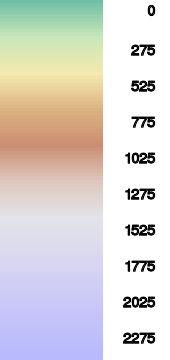
\includegraphics[angle=0,width=3.0cm,keepaspectratio='true']{figures/ramp-terrain-flatlands.png}&
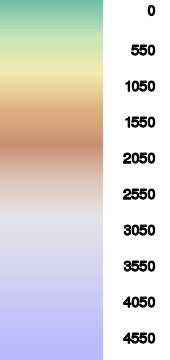
\includegraphics[angle=0,width=3.0cm,keepaspectratio='true']{figures/ramp-terrain-mountanous.png}&
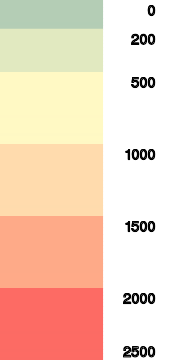
\includegraphics[angle=0,width=3.0cm,keepaspectratio='true']{figures/ramp-terrain-icao.png}&
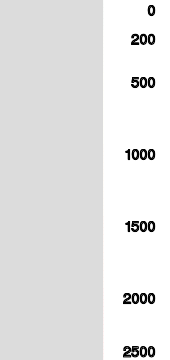
\includegraphics[angle=0,width=3.0cm,keepaspectratio='true']{figures/ramp-terrain-grey.png}
\end{longtable}

\begin{longtable}{c c c c}
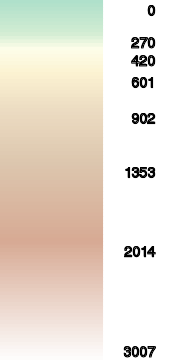
\includegraphics[angle=0,width=3.0cm,keepaspectratio='true']{figures/ramp-terrain-imhof4.png}&
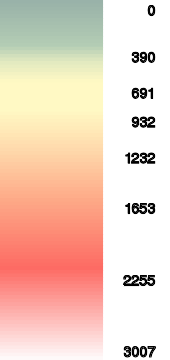
\includegraphics[angle=0,width=3.0cm,keepaspectratio='true']{figures/ramp-terrain-imhof7.png}&
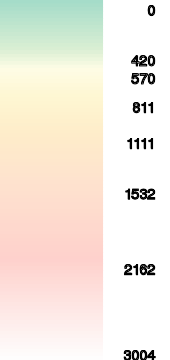
\includegraphics[angle=0,width=3.0cm,keepaspectratio='true']{figures/ramp-terrain-imhof12.png}&
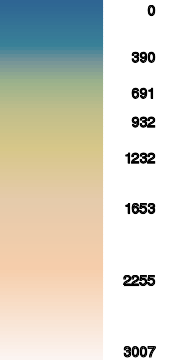
\includegraphics[angle=0,width=3.0cm,keepaspectratio='true']{figures/ramp-terrain-imhofatlas.png}
\end{longtable}


%%%%%%%%%%%%%%%%%%
\section{Kartenanzeige / Luftraum}\label{sec:airspace-display}

Hier kann die Darstellung von Lufträumen und mögliche Vorwarnzeiten
 beeinflußt werden.

\begin{description}
\item[\textit{Luftraumanzeige}]  Hier können die Anzeigemodi für die Lufträume in
Abhängigkeit von der Höhe konfiguriert werden.
Die Luftraumfilter ermöglichen ebenfalls das Filtern von Lufträumen und Warnungen für jede
\sketch{figures/config-airspace.png} einzelne Luftraumklasse. \\
  {\bf Alles Ein}: Es werden alle Lufträume angezeigt.\\
  {\bf bis max. Höhe}: Nur die Lufträume unterhalb dieser einstellbaren Höhe werden dargestellt.\\
  {\bf Auto}: Alle Lufträume in einem konfigurierbarem Höhenband um das Luftfahrzeug herum werden angezeigt.
\\
  {\bf Alles unter mir}:  Wie ''Auto'', aber Anzeige sämtlicher Lufträume unterhalb des Flugzeuges.
\item[\textit{Warnungen}]  {\bf Ein /Aus}:  Einschalten oder Abschalten der Warnungen für Lufträume.
\item[\textit{Vorwarnzeit$^{\textcolor{blue}{\star}}$}]  {\bf sec, min}: Einstellbare Zeit für vorhergesagten Luftraumeintritt, zu der eine Warnung erfolgen wird.
\item[\textit{Bestätigungszeit$^{\textcolor{blue}{\star}}$}]  {\bf sec, min}: Für diese Zeit wird die Weiderholung einer Luftraumwarnung ausgesetzt.
\item[\textit{Benutze schwarze Kontur$^{\textcolor{blue}{\star}}$}] Zeichnet einen schwarzen Rahmen um jeden Luftraum anstelle der entsprechenden Luftraumfarbe
\item[\textit{Luftraum Füllmodus$^{\textcolor{blue}{\star}}$}]  {\bf }:  Hier kann definiert werden, wie die Lufträume gefüllt werden.\\
   {\bf Voreinstellung}: Sucht anhand der Geräteperformance automatisch die beste Art der Darstellung heraus.
    Normalerweise wird hier --bis auf das PPC2000-Betriebsystem-- der Füllmodus ''Rahmen'' bevorzugt.\\
    {\bf Ganz ausfüllen}:  Transparently fills the airspace colour over the whole area. \\
    {\bf Rahmen}: Zeichnet einen satten Rahmen um den halbtransparenten Luftraum. \\
%\item[Luftraumtransparenz$^{\textcolor{blue}{\star}}$]  {\bf Ein /Aus}: Wenn eingeschaltet, dann werden Lufträume transparent dargestellt.
% nicht mehr seit 6.6
\end{description}

Auf dieser Seite gibt es am unteren Rande zwei weitere Schaltflächen  \button{Filter} und
 \button{Farben} mit denen für jede einzelne Luftraumklasse Farbe, Rahmen und Muster
 eingestellt werden kann.
 Außerdem ist möglich in den Filtereinstellungen die Sichtbarkeit zu regulieren/festzulegen.
Abhängig von der Hardware kann es sein, daß nicht alle Transparenzeigenschaften gezeigt
werden können.

\subsection*{Farben}
Mit dieser Funktion wird die Farbe, Rahmen des Luftraumes,  Dicke des Rahmens und
anderes eingestellt.

Zuerst einen Luftraum auswählen, dann doppelkicken und mit \button{Farbe der Umrandung}  bzw.
\button{Füllfarbe ändern} die gewünschten Eigenschaften zuordnen.

\subsection*{Filter}
Die Filterfunktion ist beschrieben in Kap.~\ref{sec:airspace-filter}.


%%%%%%%%%%%%%%%%%%
\section{Endanflugrechner/Sicherheitsfaktoren}
Hier werden Einstellungen für die Sicherheitshöhen und deren Verhalten in den Berechnungsalgorythmen vorgenommen.

\begin{description}
\item[\textit{Ankunftshöhe}] Sicherheitshöhe. \index{Sicherheitshöhe!Einstellung} Diese  gibt die Höhe über Grund am Zielpunkt an, in der das
Flugzeug für eine sichere Landung ankommen sollte. Gesetzt auf Null bedeutet, daß man am Zielplatz in Null Meter Höhe ''aufschlägt''.
\item[\textit{Geländefreiheit}]  \label{conf:safetyterrain} Sicherheitshöhe. Eine einstellbare Höhe, die das Flugzeug während des Endanfluges
\sketch{figures/config-safety.png}nicht unterschreiten sollte. Vermeidet damit ''in den Berg fliegen'', da \xc dann vorschlägt weiter zu Kurbeln. (Man kann natürlich auch
drumherum fliegen\dots mit dem Rotenplaner\dots)\\
Mehr zu Sicherheitshöhen, deren Bedeutung und Definition  im Kapitel~\ref{sec:safety-heights}.
\item[\textit{Alternativen Modus}]  \label{conf:alternatesmode} Bestimmt, wie beim Abbruch einer Aufgabe die Wegpunktalternativen
innerhalb des Wegpunktdialoges sortiert und vorgeschlagen werden. \\
{\bf Einfach}: Die Alternativen werden nur Ankunftshöhe sortiert ausgegeben. Der erste Punkt auf der Liste ist der nächstliegende
und preferierte.\\
{\bf Aufgabe}: Die Sortierung berücksichtigt  zusätzlich die Kursrichtung, sodaß der nächstgelegene Platz in Kursrichtung
preferiert wird. \\
{\bf Heimat}:  Ähnlich wie die ''Aufgabe''-Sortierung, aber  mit dem \textsl{Heimatplatz} als Bezugskurs.   Diese Sortierung berücksichtigt
auch Wegpunktalternativen in Richtung des konfigurierten \textsl{Heimatplatzes}  - welcher \textsl{nicht unbedingt der Startpunkt} sein muß \achtung
\item[\textit{Polaren Verschlechterung$^{\textcolor{blue}{\star}}$}] Einstellung für eine permanente Verschlechterung der Polare. Einstellung auf $0 \% $ bedeutet keine Verschlechterung,
$50 \% $ bedeutet, daß die Sinkrate \textbf{verdoppelt} ist (!)\index{Polare!Auswirkung des Faktors}
\item[\textit{Sicherheits MC$^{\textcolor{blue}{\star}}$}]  Wenn Sicherheits MC aktiviert ist, dann wird dieser Wert \textit{nach einem Abbruch einer Aufgabe} für die Kalkulation von Reichweite, Alternativen und Ankunftshöhen an Flugplätzen und Landefeldern benutzt.\label{safety-MC} 

\item[\textit{Vorflug Risikofaktor$^{\textcolor{blue}{\star}}$}]
 Der Vorlfugrisikofaktor reduziert den MC-Wert für die Vorfluggeschwindigkeit mit fallender Flughöhe um das Risko einer
 Außenlandung zu mindern. Wenn zu $0,0$ gesetzt, bedeutet dies keine Anpassung an die aktuelle Flughöhe, gesetzt auf $1,0$
wird der MC Wert linear bezogen auf die aktuelle Höhe reduziert, als Bezugspunkt gilt dabei die maximal während des
Fluges erreichte Höhe.
Ein Wert von ca. $0.3$ ist empfohlen.  Mehr dazu auch in Kap.~\ref{sec:safety-factor}.
\end{description}


%%%%%%%%%%%%%%%%%%
\section{Endanflugrechner / Endanflugrechner}\label{sec:final-glide}
Über diese Seite können die Routinen des Endanflugrechners von \xc  beinflußt werden.

\begin{description}
\item[\textit{MC Optimierung}]  Diese Option setzt fest, welcher MC-Algorythmus verwendet wrd.
Mehr dazu in Kap.~\ref{sec:auto-maccready}. \\
   {\bf Endanflug}: Stellt den MC Wert auf die schnellstmögliche Ankunft ein.
   Bei OLC - Aufgaben werden die Einstellungen  so gewählt, daß \sketch{figures/config-glidecomputer.png} eine möglichst große Strecke innerhalb der verbleibenden Zeit zurückgelegt wird.\\
   {\bf Erwartetes mittleres Steigen}: Die MC Einstellungen basierend auf den bisher ermittelten Steigwerten gesetzt.\\
   {\bf Beides}: Benutzt ''Erwartetes mittleres Steigen'' während der Aufgabe und wechselt im Endanflug automatisch auf  ''Endanflug''.
\item[\textit{Blockgeschwindigkeit$^{\textcolor{blue}{\star}}$}] {\bf Ein / Aus}: Wenn eingeschaltet, wird die Sollfahrt für den Vorflug empfohlen, welche für Gleiten ohne vertikale Luftbewegung gilt.
Andern falls werden die Sollfahrten nach dem Delphin-Stil vorgeschlagen, es wird dann die vertikale Luftbewegung mit in die Sollfahrtberechnung
einbezogen.
\item[\textit{Nav. mit barometrischer Höhe$^{\textcolor{blue}{\star}}$}] {\bf Ein / Aus}: Wenn eingeschaltet und ein barometrischer Höhenmesser angeschlossen ist, dann wird die barometrische Höhe für alle Navigationsfunktionen verwendet. Ansonsten wird die GPS--Höhe benutzt.
\item[\textit{Wechsel Steig-/Vorflugmodus$^{\textcolor{blue}{\star}}$}] {\bf Ein / Aus}: Wenn ein Vega Variometer angeschlossen ist und diese Option aktiviert ist, wird mit der Wölbklappe zwischen Kreis- und Vorflug umgeschaltet.
Das bedeutet, daß  beim Umwölben sofort der entsprechende Modus aktiviert wird (auch beim Borgelt B50 verfügbar)
\item[\textit{Gleitzahl Mittelwertzeitintervall$^{\textcolor{blue}{\star}}$}] {\bf sec, min}: Hier kann entscheiden werden, welche Zeitspanne für die Mittelwertbildung benutzt werden soll.
Die Mittelwertbildung wird grundsätzlich in Echtzeit vorgenommen. Berechnet wird das erreichte Höhen zu Streckenverhältnis
innerhalb der hier ausgewählten Zeitspanne.

Wenn Du zum Beispiel wegfliegst und nach zwei Minuten zum gleichen Punkt zurückkehrst und Du hast eine Zeitspanne von zwei Minuten eingestellt,
dann nimmt der Integrator die Strecke innerhalb dieser zwei Minuten annehmen, welche aber dann Null (Punkt A = Punkt B $\Rightarrow \bar{AB} = 0$ )
ist und somit wird die Gleitzahl auch Null.

Normalerweise ist für Segelflugzeuge ein Wert von 90 - 120 sec.\ zu bevorzugen,
für Paragleiter sind 15 sec.\ OK. Kleinere Werte werden als Ergebnis immer näher an den
aktuellen Wert herankommen, größere Werte immer weiter an den Wert gemittell über den gesamten Flug.
(Klar, bei einer Mittelwertbildung\dots) Andere kommerziell erhältliche Instrumente benutzen Werte von ca. 120 Sekunden.
\item[\textit{Geschätzte Winddrift$^{\textcolor{blue}{\star}}$}]  {\bf Ein / Aus}: Berücksichtigt die Abdrift durch den Wind während des Kurbelns. Dies wird die Ankunftshöhe auf Gegenwindschenkeln reduzieren
und kann mitunter zu interpretationswürdigen Ergebnissen führen,
wenn man sich im Endanflug unterhalb des Gleitpfades befindet, MC auf Null gestellt hat, und so also noch kurbeln \textsl{muß}.
Nach der MC-Theorie heißt MC=0, daß kein Kurbeln mehr stattfindet. Der Algorythmus befindet sich so in einer Zwickmühle, denn einerseits wird mitgeteilt, daß nicht
mehr gekurbelt wird, andererseits tut man es doch\dots
\achtung Für das ''normale, althergebrachte Verhalten'' anderer Systeme sollte man sich überlegen, dies auf ''Aus'' stehen zu lassen.
\end{description}


%%%%%%%%%%%%%%%%%%
\section{Endanflugrechner / Wind} \label{sec:final-wind}
Auf dieser Seite werden die Windeinstellungen vorgenommen. Details zu den verschiedenen Berechnungen in Kap.~\ref{sec:wind-estimation}
\begin{description}
\item[\textit{Windberech}]  \label{conf:autowind}  Auswahl des entsprechenden modus für Ermittlung des Windes in \xc \\
  {\bf Manuell}: Wenn der Algorythmus ausgeschaltet ist, wird allein die Eingabe des Piloten benutzt. \\
  {\bf beim Kreisen}: Benutzt das GPS zur Ermittlung des Windes durch Berechnung der Abdrift beim Kurbeln.\\
  \sketch{figures/config-wind.png}{\bf ZickZack}: ZickZack-Modus benötigt ein intelligentes Vario  mit einem Ausgang für die TAS.\\
  {\bf Beides}:  Benutzt den ZickZack und GPS-Modus zur Ermittlung des Windes.
\item[\textit{Externer Wind}]  Wenn eingeschaltet und ein entsprechendes gerät am \xc angeschlossen ist, dann wird der Wind von einem
externen Gerät in die internen Routinen übernommen.
\end{description}


%%%%%%%%%%%%%%%%%%
\section{Endanflugrechner / Routenplaner}\label{sec:final-route}
Seite für die Einstellungen für die Reichweite und Routenplaner-Optimierungen.

\begin{description}
\item[\textit{Routenplaner Modus}]  \label{conf:routemode} {\bf Keine, Gelände, Luftraum, Beides}
  Einstellung, welcher Modus für die Routenplanung benutzt werden soll. Für Details bitte in Kap.~\ref{sec:route} nachschauen.
\item[\textit{Pfadsuche mit Steigen$^{\textcolor{blue}{\star}}$}]  {\bf Ein / Aus}: \label{conf:routeclimb} Wenn dies aktiviert und MC größer Null, dann erlaubt der Routenplaner
  Steigphasen zwischen der aktuellen Position und dem Ziel.
\item[\textit{Wolkenuntergrenze$^{\textcolor{blue}{\star}}$}]  \label{conf:routeceiling}{\bf Ein / Aus}:  Wenn aktiviert wird bei der Routenplanung  das Steigen durch die Wolkenbasis begrenzt. Sie wird mit 500 m über der momentanen Flugzeughöhe und der Thermikhöhe angenommen.
  Wenn nicht aktiviert wird mit unbegrenztem Steigen geplant.
\sketch{figures/config-route.png}
\item[\textit{Reichweiten Modus}]  \label{conf:turningreach} Die Reichweitenberechnung kann Umwege durch vorhandene Hindernisse berücksichtiegn.
  Hier werden die Einstellungen dazu vorgenommen:\\
  {\bf Aus}: Reichweite wird nicht berechnet.\\
  {\bf Direkt}: Reichweite wird in geradem Weg vom Flugzeug aus berechnet.\\
  {\bf Mit Umweg}: Die Reichweitenberechnung wird unter Berücksichtigung von Hindernissen vorgenommen.
\item[\textit{Erreichbare Anzeige}]  \label{conf:gliderange} Einstellung, wie die Reichweite auf der moving map dargestellt wird.\\
  {\bf Aus}: Keine Darstellung des Gleitbereiches.\\
  {\bf Grenzlinie }:Zeichnet eine gestrichelte linie um den aktuell erreichbaren Bereich.\\
  {\bf Schattiert }: Verdunkelt das Gelände außerhalb der aktuellen Reichweite etwas
\item[\textit{Erreichbare Polare$^{\textcolor{blue}{\star}}$}]  \label{conf:reachpolar}
   Einstellung der Gleiteigenschaften des Flugzeuges für die Berechnung von Reichweite, Ankunftshöhen, Aufgabenabbruch und alternativen Landeplätzen.\\
  {\bf Aufgabe}: Verwendet den Mc-Wert aus der Aufgabe\\
  {\bf Sicherheits MC}: Verwendet den eingegebenen Sicherheits-Mc-Wert.
\end{description}


%%%%%%%%%%%%%%%%%%
\section{Anzeigen / FLARM, etc.} \label{sec:flarmandother-gauge}

\begin{description}
\item[\textit{FLARM Radar}]  \label{conf:flarmdisplay} {\bf Ein / Aus}: \\
{\bf Ein}: Aktiviert die Anzeige des FLARM Radars. Die Flugrichtung des Ziels relativ zum eigenen Steuerkurs wird als Pfeilkopf dargestellt.
Ein Dreieck, das nach oben oder nach unten zeigt die Höhe des Zieles relativ zur Eigenen an.
\sketch{figures/flarmrose.png}\\
{\bf Aus}: Flarmanzeige des Luftverkehrs  bleibt aus.
\item[\textit{Schließe FLARM automatisch$^{\textcolor{blue}{\star}}$}] {\bf Ein / Aus}: \\
{\bf Ein}: Eingeschaltet, wird der FLARM Dialog automatisch geschlossen, sobald kein Verkehr da ist.\\
{\bf Aus}: Beläßt den Dialog offen, auch wenn kein Verkehr mehr da ist.
\item[\textit{Zentrierhilfe}] \label{conf:thermalassistant} {\bf Ein / Aus}: \\
{\bf Ein}: Aktiviert die Anzeige des Thermikassistenten (Zentrierhilfe).\\
{\bf Aus}: Keine Zentrierhilfe.
\item[\textit{Thermikprofil}] \label{conf:thermalband} {\bf Ein / Aus}: \\ 
{\bf Ein}: Aktiviert die Anzeige des Thermikprofils am linken oberen Rand der Karte\\
{\bf Aus}: Keine Anzeige
\item[\textit{Endanfluganzeige für MC 0$^{\textcolor{blue}{\star}}$}] {\bf Ein / Aus}:\\
{\bf Ein}: Wenn aktiviert zeigt der Endanflug--Anzeigepfeil eine zusätzlichen, zweiten, längs halbierten Pfeil für die bei MC 0 Einstellung benötigte Höhe 
um das Ziel zu erreichen.\\
{\bf Aus}: Es gibt nur einen vollen Pfeil
\end{description}

In allen Modi deutet die Farbe des Zieles auf den Level der potentiellen Gefahr an (grün, gelb, rot\dots)


%%%%%%%%%%
\section{Anzeigen / Vario}\label{sec:vario-gauge}

Hier können \textsl{dezimale Anzeigen} auf dem Vario-Anzeige-Bereich  ein- und ausgeschaltete werden.
Mithilfe des Zeigers (ganz unten) kann auch ein Mittelwert-Zeiger an oder ausgeschaltet werden,
\index{Vario!Elemente} diesen auf der analogen Ringdarstellung zu platzieren.\index{Vario!Aussehen}
\begin{description}
\item[\textit{Geschwindigkeitspfeile$^{\textcolor{blue}{\star}}$}]  \label{conf:variogauge} Ob Pfeile für die Sollfahrt  in der Varioanzeige dargestellt werden sollen.\\
{\bf Ein}: Wenn aktiviert weisen im Vorflugmodus  Aufwärtspfeile zum langsamer Fliegen (Ziehen--nach oben ) an,  Abwärtspfeile zum schneller Fliegen an (Drücken--nach unten).
\sketch{figures/config-othergauges.png}{\bf Aus}:  KeineAnzeige.\\
\item[\textit{Zeige Mittelwert$^{\textcolor{blue}{\star}}$}]  {\bf Ein / Aus}: Ob das mittlere Steigen angezeigt werden soll.
Im Vorflug wird auf mittlere Nettovario Anzeige geschaltet.
\item[\textit{Zeige MacCready$^{\textcolor{blue}{\star}}$}] {\bf Ein / Aus}: Anzeige des  MacCready-Wertes  ein oder aus.
\item[\textit{Zeige Mücken$^{\textcolor{blue}{\star}}$}] {\bf Ein / Aus}: Anzeige der Mückenbeladung in Prozent.
\item[\textit{Zeige ballast$^{\textcolor{blue}{\star}}$}] {\bf Ein / Aus}:Anzeige des Wasserballast ein oder aus. Anzeige in Prozent.
\item[\textit{Zeige brutto$^{\textcolor{blue}{\star}}$}] {\bf Ein / Aus}: Anzeige des Bruttosteigens ein oder aus.
\item[\textit{Mittelwert Zeiger$^{\textcolor{blue}{\star}}$}] {\bf Ein / Aus}: Falls aktiviert ist in der Varioanzeige eine hohle Mittelwertnadel zu sehen.
Im \textsl{Vorflug} zeigt diese Nadel das gemittelte Nettovario,
beim \textsl{Kurbeln} wird das mittlere Bruttovario angezeigt.
\end{description}

%%%%%%%%%%
\section{Anzeigen / Audio-Vario}\label{sec:audiovario-gauge}

Hier werden Einstellungen für die Tonausgabe des Varios vorgenommen.\index{Vario!Tonausgabe}
\label{conf:audiovariogauge}

\begin{description}
\item[\textit{Tonvario}]  {\bf Ein / Aus}:  Ein oder Ausschalten der Tonausgabe des Varios
\item[\textit{Volumen}]  Einstellung der Laustärke.
\item[\textit{Tonausblendung Ein}]  {\bf Ein / Aus}: Unterdrückung der Tonausgabe, wenn das TEiegn (oder Sinken) innerhalbeines betimmten Wertes um Null ist.
\item[\textit{Niedrigster Ton$^{\textcolor{blue}{\star}}$}]  Frequenz des Tones bei größtem Saufen.
\sketch{figures/config-audiovario.png}
\item[\textit{Null-Ton$^{\textcolor{blue}{\star}}$}]  Frequenz des Tones bei Nullschieber.
\item[\textit{Höchster Ton$^{\textcolor{blue}{\star}}$}]  Frequenz des Tones bei größtem Steigen.
\item[\textit{Tonausblendung min. Steigen$^{\textcolor{blue}{\star}}$}]  Wenn die Tonausblendung aktiviert ist, gibt das Vario unterhalb dieses Grenzwertes Töne aus.
\item[\textit{Tonausblendung max. Steigen$^{\textcolor{blue}{\star}}$}]  Wenn die Tonausblendung aktiviert ist, gibt das Vario oberhalb dieses Grenzwertes für das Steigen Töne aus.
\end{description}


%%%%%%%%%%%%%%%%%%
\section{Aufgabenvoreinstellungen / Regeln}

Auf dieser Seite werden Regeln für Aufgaben global voreingestellt.
rules. \label{conf:taskrules}\index{Aufgabe!Regeln Voreinstellung}

\begin{description}
\item[\textit{Max. Abfluggeschwindigkeit$^{\textcolor{blue}{\star}}$}] Einstellung der maximalen Abfluggeschwindigkeit über die deklarierte Abfluglinie.
   Wenn kein Limit vorgegeben ist, sollte der Wert auf $0$ gesetzt werden.
\item[\textit{Max. Abflug-Geschwindigkeitstoleranz$^{\textcolor{blue}{\star}}$}] Maximal tolerierte Geschwindigkeitstoleranz der vorgegebenen Abfluggeschwindigkeit.
   Für Null-Toleranz zu $0$ setzen.
\item[\textit{Maximale Abflughöhe$^{\textcolor{blue}{\star}}$}]  Maximale Abflughöhe bei Überfliegen der Abfluglinie.
   (MSL oder GND möglich--s.u.) Für Start ohne Höhenbegrenzung zu $0$ setzen.
\item[\textit{Max. tolerierte Abflugüberhöhung$^{\textcolor{blue}{\star}}$}]  Maximal tolerierte Höhe über der vorgegebenen Abflughöhe
   Wenn keine Toleranz erlaubt, zu $0$ setzen.
\sketch{figures/config-rules.png}
\item[\textit{Abflughöhe bezogen auf$^{\textcolor{blue}{\star}}$}]  Bezugshöhe der max. Abflughöhen:\\
    {\bf MSL}: Abflughöhe ist bezogen auf Meereshöhe.\\
    {\bf AGL}: Abflughöhe ist bezogen auf Höhe über Grund.
\item[\textit{Min. Ankunftshöhe$^{\textcolor{blue}{\star}}$}]  Minimale Ankunftshöhe zum Überqueren der Ziellinie / Zielkreises
    (AGL or MSL). Wenn keine Abweichung erlaubt ist, zu $0$ setzen.
\item[\textit{Zielhöhenref.$^{\textcolor{blue}{\star}}$}] Bezugshöhe der Ankunftshöhe:\\
    {\bf MSL}: Ankunftshöhe ist bezogen auf Meereshöhe.\\
    {\bf AGL}: Ankunftshöhe ist bezogen auf Höhe über Grund.
\item[\textit{On-Line Contest}]  Einstellungen zu den Optimierungsalgorythmen des OLC.
   Die Implementierung enstpricht der ofiziellen Ausgabe vom 23. September 2010. \\
   {\bf OLC FAI}: Gleichlautend zu den FAI-Dreiecksregeln. Zwei Wenden, wobei Star-und Zielpunkt identisch sind.
   Kein Schenkel darf kürzer sein als 28\% der Gesamtstrecke. Bei Dreiecken größer als 500Km
   darf kein Schenkel größer sein als 25\% der Gesamtstrecke und länger als 45\% andernfalls kein
   Schenkel kleiner als 28\%. Ankunftshöhe darf nicht  tiefer sein als Starthöhe -1000m.\\
   {\bf OLC Classic}: Bis zu sieben Punkte einschließlich Start und Ziel, Ankunftshöhe nicht
   mehr als 1000m unter der Abflughöhe. \\
   {\bf OLC League}: Der aktuelle Contest mit Sprint-Wettbewerbsregeln.
   Aus dem OLC Classic Dreieck wird das 2,5 Stunden Fenster mit dem besten Schnitt herausgschnitten. 
   Ankunftshöhe darf nicht unter Abflughöhe liegen.\\
  {\bf OLC Plus}: Kombination aus Classic und FAI Regeln. 30\% der FAI Punkte werden zur
   Classic Wertung dazugezählt \\
  {\bf XContest}: \todonum{noch zu schreiben} \\
  {\bf DHV-XC}: \todonum{noch zu schreiben} \\
  {\bf SIS-AT}: \todonum{noch zu schreiben} \\
  {\bf FFVV NetCoupe}: Der FFVV NetCoupe {\it ''libre''} Wettbewerb.
\item[\textit{Wertungs-Vorhersage}]  {\bf Ein / Aus}: Wenn eingeschaltet, wird angenommen, daß der nächste Wegpunkt erreicht wird und
die daraus sich ergebende Wertung errechnet.
\end{description}


%%%%%%%%%%%%%%%%%%
\section{Aufgabenvoreinstellungen  / Wendepunkttypen}

Einstellungen für Start, Ziel und Wendepunkte können hier global konfiguriert werden.
Diese Werte werden bei Erstellung einer neuen Aufgabe als Standard genommen.
Die Feineinstellung  ist im Aufgabeneditor vorzunehmen.
Mehr dazu in Kap~\ref{cha:tasks}. \index{Aufgabe!Regeln!Voreinstellungen}


\begin{description}
\item[\textit{Startpunkt}] Standard Einstellungen für neu zu erstellende Aufgaben.\\
{\bf  Abfluglinie}: Ein geradliniges Tor. Wird auf der Map mit einem Halbkreis entgegengesetzt zum ersten Schenkel
dargestellt. Überquere diese Linie entsprechend der Aufgabenvorgaben aus dem Sektor heraus.\\
{\bf  Abflugzylinder}: Ein Zylinder um den Startpunkt herum. Von innen nach außen überfliegen.\\
{\bf FAI-Abflug-Quadrant}: Ein 90$^\circ$ Sektor mit 1km Radius. Überfliege de Flanken vom inneren her für den Abflug.\\
{\bf  BGA Abflugsektor}:Ein 180$^\circ$ Sektor mit 5km Radius. Verlasse den Sektor in irgendeine Richtung für den Abflug.
\item[\textit{Torbreite}] Standard Radius oder Torbreite in Km für neu zu erstellende Aufgaben.
\item[\textit{Zielpunkt}] Standard Ziel-Typ für neu zu erstellende Aufgaben.\\
{\bf Ziellinie}: Überfliege diese Linie nach Vorgabe der WB-Leitung.\\
{\bf Zielzylinder}: Fliege in diesen Zylinder.\\
{\bf FAI Zielquandrant}: Ein 90$^\circ$ Sektor mit 1Km Radius. Überfliege die flanken für gültigen Einflug.
\item[\textit{Radius}] Standard Radius oder Torbreite in Km für neu zu erstellende Aufgaben.
\item[\textit{Wendepunkt}] Standard Wendepunkt-Typ für neu zu erstellende Aufgaben.\\
{\bf Wendepunkt-Zylinder}: Ein Zylinder. Ein Punkt im Zylinder gilt als gültig, gewertet wird der Mittelpunkt\\
{\bf Schlüssellochsektor (DAEC)}: Jeder Punkt innerhalb eines 500m Zylinders vom Zentrum oder 10Km innerhalb
des 90$^\circ$ Sektors. Gewertet wird der Mittelpunkt.(deustch)\\
{\bf BGA festgelegter Kurssektor}: Jeder Punkt innerhalb 500m Zylinder, oder 20Km  in einem 90$^\circ$ Sektor.
Gewertet wird das Zentrum des Zylinders.(britisch)\\
{\bf BGA Erweiterungsoption festgelegter Kurs}:Jeder Punkt innerhalb 500m Zylinder, oder 10Km  in einem 180$^\circ$ Sektor.
Gewertet wird das Zentrum des Zylinders.(britisch)\\
{\bf FAI Quadrant}: Ein 90$^\circ$ Sektor mit unendlicher Seitenlänge. Überfliege eine Flanke. Gewertet wird vom Eckpunkt.
\item[\textit{Radius}] Standard Radius oder Torbreite in Km für neu zu erstellende Aufgaben.
\item[\textit{Aufgabe}] Standard Aufgaben-Typ für neu zu erstellende Aufgaben.\\
{\bf Racing }:Geschwindigkeitsaufgabe um Wendepunkte. Kann für FAI Abzeichen oder auch Rekordversuche  verwendet werden. Alle OZ-Typen sind möglich.\\
{\bf  AAT}: Geschwindigkeitsaufgabe über zugeweisene Gebiete. Mindestflugzeit wird vorgegeben. Beschränkt auf Zylinder und Sektorgebiete. Gewertet wird bester Schnitt.\\
{\bf  FAI Abzeichen / Rekorde}: FAI-Regeln. Erlaubt nur FAI Start-, Ziel- und Wendepunkttypen. Für Abzeichen und Rekorde. Aktiviert die FAI Höhe für die Endanflugbnerechnung.
\item[\textit{AAT min. Zeit}] Die bei AAT-Aufgaben mindestens zu fliegende Zeit. Vorgabe durch WB-Leitung.
\item[\textit{Optimierungs-Spielraum$^{\textcolor{blue}{\star}}$}] Sicherheitszeitraum für AAT-Optimierung.
Als Schutz gegen ''zu früh ankommen''. Der Optimierungsalgorythmus versucht, die Aufgabe innerhalb der vorgegebenen Mindestflugzeit plus dieser Zusatzzeit zu bneenden.
Im ''Optimiert''-Modus  werden dabei die AAT-Punkte automatisch verschoben, um diese Zeit einhalten zu können..
\end{description}


%%%%%%%%%%%%%%%%%%
\section{Aussehen / Sprache, Eingaben}\label{sec:interface}

Auf dieser Seite können Interaktionen und Aussehen der Menüs von \xc beeinflußt werden.


\begin{description}
%\item[Auto Blank\textcolor{blue}{$\star$}]  This determines whether to blank the display after a long
%  period of inactivity when operating on internal battery power (visible for some mobile
%  devices only).
\item[\textit{Ereignis$^{\textcolor{blue}{\star}}$}]  Die Eingabeereignisdatei bestimmt, wie \xc auf bestimmte Eingaben wie z.B.\ einen Knopfdruck oder einer
Eingabe eines externen Gerätes reagiert.
\item[\textit{Sprache}]  Die Sprache (2 stellige Abkürzungen als Auswahl) der Oberfläche -- übersetzt aus dem Englischen.
{\bf Automatisch} wählt die Sprache anhand der Betriebssystemeinstellung aus.
\item[\textit{Nachricht$^{\textcolor{blue}{\star}}$}] Die Statusdatei legt fest, welche Klänge auf welche Ereignisse hin abgespielt werden
und wie lange die verschiedenen Meldungen auf dem Bildschirm sichtbar bleiben.
\item[\textit{Menü Zeitabschaltung$^{\textcolor{blue}{\star}}$}] Diese Zeit bestimmt, wie lange ein Menü ohne weitere Eingabe des Benutzers auf
dem Bildschirm sichtbar bleibt, bevor es wieder ausgeblendet wird.
\item[\textit{Texteingabestil$^{\textcolor{blue}{\star}}$}]  Auswahl, wie Text eingegeben werden kann. Es stehen drei Möglichkeiten zur Auswahl:
  Siehe hierzu Kap.~\ref{sec:textentry} für mehr Info dazu. \\
    {\bf Voreinstellung}: Die Standardeinstellung des Betriebsystemes des Gerätes wird benutzt.\\
    {\bf Tastatur}: Benutzt eine Bildschirmtastatur  für die Eingabe.  \\
    {\bf Ranglisten Stil}: Auswahl von Buchstaben durch unterstrichenen blinkenden Cursor.
\item[\textit{Haptische Rückmeldung$^{\textcolor{blue}{\star}}$}]  {\bf Ein / Aus}: (Nur bei Android Geräten) Schaltet die Vibration des Gerätes bei Berührung der TouchScreen-Oberfläche  ein oder aus. Das ist das ''\texttt{brrt..}''\dots
\end{description}



Um die Schriften von \xc anzupassen, drücke auf den hier vorhandenen  \button{Schriften} Knopf.

\subsection*{Schriften}\index{Schriften!Anpassen}

Auswahl der verschiedenen Schriften für diverse Anzeigeelemente. Anwahl des beschriebenen
Elementes und Auswahl der dazu angebotenen Schrift, -größe und -format.


Falls nicht vom Benutzer konfiguriert, werden voreingestellte Standardschriften verwendet.
\sketch{figures/config-fonts.png}


%%%%%%%%%%%%%%%%%%
\vspace{5em}
\section{Aussehen / Anordnung}\label{sec:interface-appearance}

Auf dieser Seite können weitere Details zum look and feel der Oberfläche
angepaßt werden.


\begin{description}
\item[\textit{InfoBox Geometrie}]  Eine Auswahlliste von mehreren Anordnungen der InfoBox Seiten Je nach Gerät und persöhnlichem
Geschmack muß dies schlicht ausprobiert werden. Die angebene Zahl entspricht der Anzahl der InfoBoxen auf der entsprechenden InfoBoxSeite.
\item[\textit{FLARM Anzeige$^{\textcolor{blue}{\star}}$}]  \label{conf:flarmradar-place}
Wen das \fl angeschaltet wird, kannst Du das kleine \fl Radar es hiermit an entsprechenden stellen einer InfoBoxSeite plazieren.
Als Standard ist ein ''Auto''-Setup vorhanden, was bedeutet, daß das Radar lediglich die InfoBoxen
überlappt und nicht einen Teil der MovingMap.
\item[\textit{Reiter Dialogstil}] Einstellung, ob Icons oder Text auf beschrifteten Seiten angezeigt werden sollen.
Bspw. im Aufgaben Editor.
\item[\textit{Nachrichtenanzeige$^{\textcolor{blue}{\star}}$}]  Einstellung, wo Nachrichten und Systemmeldungsfenster
erscheinen sollen.   {\bf Zentriert} oder in der {\bf Oben Links} Ecke.
\item[\textit{Dialogfenstergröße$^{\textcolor{blue}{\star}}$}]  Einstellung über die Größe der Dialogfenster{\bf Volle Breite},  {\bf Skaliert},  {\bf Skaliert und zentriert} und {\bf fixiert} stehen zur Auswahl.
\item[\textit{Invertierte InfoBox$^{\textcolor{blue}{\star}}$}]  Wenn {\bf Ein}, werden die InfoBoxen weiß auf schwarzem Hintergrund, wenn {\bf Aus} schwarz auf weißem Hintergrund dargestellt.
\item[\textit{Farbige InfoBoxen$^{\textcolor{blue}{\star}}$}]  Wenn {\bf On}, haben manche InfoBoxen farbige Inhalte. Wenn {\bf Aus}, erfolgt die Darstellung in Schwarz/Weiß.
Zum Beispiel wird der aktive Wegpunkt-InfoBox  blau dargestellt, wenn sich das Flugzeug oberhalb des Gleitpfades für den Endanflug  befindet,
\item[\textit{InfoBox Rahmen$^{\textcolor{blue}{\star}}$}]  Es gibt zwei Arten, die InfoBoxen zu umrahmen:\\
  {\bf Kasten}: Zeichnet einen Kasten um jede InfoBox.\\
  {\bf Tab}: Zeichnet einen Reiter über den Titel der InfoBox
  title. \\
\end{description}


%%%%%%%%%%%%%%%%%%
\section{Aussehen / InfoBox Seiten (oder einfache Seiten)}

Mithilfe dieser Einstellungen kann das Aussehen und die Belegung des InfoBoxenSeiten angepaßt werden.

Es können bis zu acht InfoBoxSeiten konfiguriert und benutzt werden, da.h. es können maximal
8x8 = 64 verschiedene Infoboxen während des Fluges betrachtet werden (Ob das sinnvoll ist, sei dahin gestellt).
Eine InfoBoxSeite ist nichts anderes als eine feste Tabelle mit in verschiedenen Anordnungen eingefügten Infoboxen.

Es gibt drei vorangepasste Seiten für das Kurbeln, den Vorflug, den Endanflug eines Seite welche
nur eine Karte ganz ohne InfoBoxen zeigt und eine Automatik- InfoboxSeite, welche je nach Flugmodus
(Vorflug/Kurbeln) automatisch vom System aktiviert wird.

\begin{description}
\item[\textit{Seite  1..3}] Wähle aus, was Du meinst, was auf Deinen Seiten stehen sollte.
       Auswahl von  ''- - -'' bedeutet, daß die Seite inaktiv bleiben wird.
\item[\textit{Seite 4..8$^{\textcolor{blue}{\star}}$}]  ''Experten'' können hier weitere Seiten für Ihre Zwecke definieren
\end{description}




%%%%%%%%%%
\section{Aussehen / InfoBox Modi (und InfoBox-Sets)}\label{sec:infobox_sets}

Auf dieser Seite werden InfoBoxen-sets erstellt, geändert und konfiguriert.
Im ''Experten'' Modus können bis zu acht Sets von InfoBoxen bearbeitet werden,
in der Basis - Konfiguration lediglich vier.

Hier werden die entsprechenden InfoBoxen den entsprechenden Positionen innerhalb
der InfoBoxSeiten zugeordnet. Doppelklick auf die entsprechenden Positionen öffnet die mögliche Auswahl.

Es gibt drei vorbereitete Sets von InfoBox-Seiten
bzw. InfoBox-Seiten, welche ''beim Kurbeln'', ''Vorflug'' und ''Endanflug'' benannt sind.

\begin{description}
\item[\textit{beim Kreisen}]  vorbereitete Seite gedacht für das Kurbeln.\\
\item[\textit{Vorflug}] vorbereitete InfoBoxSeite, vorbereitet für Vorflug\\
\item[\textit{AUX-4--5}]Frei zur Verfügung stehenden InfoBoxSeiten.
\end{description}

Es können bis zu fünf weitere InfoBoxSeiten erstellt werden, welche
standardmäßig ''AUX4',''AUX5''\dots benannt sind.

Mit \button{Kopieren} ist es möglich den Inhalt der aktuellen InfoBoxSeite auf eine nächste zu übertragen.

Nach dem Anklicken öffnet sich die entsprechende Seite und kann mit den diversen InfoBoxen bestückt
und mit einem beliebigen Namen benannt werden (z.B.\ AAT-Planung) werden

\button{Endanflugmodus verwenden}  Bestimmt, ob das ''Endanflug'' InfoBox-Set für die
 ''Auto''-Seite benutzt werden soll.
%
\subsection*{InfoBox Seiten-Anpassung}\index{InfoBox!Erstellung}\index{InfoBox!Seiten}
%
\begin{description}
\item[\textit{Name}]  Hier kann ein Name für die gerade erstellte oder bearbeitete InfoBoxSeite angegeben werden.
\item[\textit{InfoBox}]  Nummer der entsprechenden Infobox innerhalb der InfoBoxSeite. (s. Tabelle weiter unten)
\item[\textit{Inhalt}]  Hier steht eine Beschreibung des aktuellen Inhaltes der schwarz hinterlegten infoBox.
\end{description}


\sketch{figures/config-infoboxset.png}

Schwarz hinterlegt ist hier die aktuell angeklickte Position der Infobox, entweder Doppelklick auf das schwarze Feld, um
den Inhalt festzulegen, oder aber anhand der vorgegebenen Numerierung vorgehen. Mehr Detail in Kap.~\ref{cha:infobox} für die genaue Beschreibung der InfoBoxen und deren Inhalt.
Die Tabelle unten zeigt einen kurzen Überblick über die Positionen der InfoBoxen im Hoch - und Querlayout.
\begin{center}\begin{multicols}{2}
\begin{tabular}{|c|c|}
\hline
1 & 7 \\
\hline
2 & 8 \\
\hline
3 & 9 \\
\hline
4 & 10 \\
\hline
5 & 11 \\
\hline
6 & 12 \\
\hline
\end{tabular}

\begin{tabular}{|c|c|c|c|}
\hline
1 & 2 & 3 & 4 \\
\hline
\hline
5 & 6 & 7 & 8 \\
\hline
\end{tabular}
\end{multicols}
\end{center}


%%%%%%%%%%%%%%%%%%
\section{Einstellung / NMEA-Anschluß} \label{conf:comdevices}\index{NMEA!Anschlüsse}\index{GPS!Liste der Geräte}\index{GPS!Treiber}

Auf dieser Seite werden die Anschlüsse der externen Geräte insbesondere der GPS-Quelle definiert und deren Parameter
angegeben. Falsche Einstellungen an dieser Stelle werden zu Fehlfunktionen führen. Es stehen ein große Menge an Gerätetreibern zur Verfügung, die aus der Auswahlliste am
oberen Rande des Fensters ausgewählt werden können.

Je nachdem, welches Gerät ausgewählt wurde, erscheinen in der unteren Hälfte des Fensters dazugehörige
Parameter zur Auswahl. \achtung Es werden daher hier alle Parameter gezeigt, unabhängig davon, ob sie bei manchen Geräten nicht erscheinen.
Die Liste ist in permanentem Wandel/Wachstum, daher kann es sein, daß nicht alle Gerät hier mit dediziertem Treibern aufgelistet sind.
Wenn das Gerät mit dem Vega verbunden werden soll, ist als Anschluß COM1 und 38400 baud zu wählen.

Standard ist COM1 und 4800 baud. Es können insgesamt 6 Geräte angeschlossen werden (Gerät A .. F).
So kann eines z.B.\ als GPS-Quelle benutzt werden und ein anderes als externes variometer.
Wenn kein weiteres Gerät angeschlossen werden soll, so ist im Auswahlfeld des entsprechenden Anschlusses ''Deaktiviert'' auszuwählen.
\xc wird diese Anschlüsse dann ignorieren und keine Zeit mit der Suche nach einem Gerät an dem Anschluß verbringen.
\sketch{figures/config-devices.png}

Es dürfen COM 0 bis 10 verwendet werden,  einschließlich einer TCP/IP Verbinung, welche z.B. für eine
Rechnerverbindung (\textsc{CONDOR} o.ä.) benutzt werden kann. Welcher COM-Port benutzt werden soll, hängt maßgeblich vom angeschlossenen Gerät ab,
welches diesen Port zur Verfügung stellt und wie es dies tut (BlueTooth, serielles Kabel, IoIo, SDCard, CF Card etc.) Auf alle diese detaillierten
Eingänge hier im Handbuch einzugehen, überstiege den Umfang des Handbuches, daher bitte auf der \xc-Hompage nachschauen, oder aber
in einer der mailing-listen  (z.B.:  im \href{http://forum.xcsoar.org/}{XCSsoar-Forum}) um Hilfe bitten.

\begin{description}
\item[\textit{Anschluß}]  Hier werden die vier möglichen Anschlüsse A..D mit dem entsprechenden Gerät belegt. (Auf das Feld gehen und anschließend entsprechenden Treiber aus Liste (s.u.) auswählen).
\item[\textit{Baudrate}]  Hier wird die Baudrate eingestellt, mit der das Programm mit den extern angeschlossenen Geräten kommuniziert.
\item[\textit{Bündel Baudrate}]  Das ist die Baudrate um Flüge zu deklarieren oder herunterzuladen (gibt es nicht bei allen Geräten).
\achtung Flarm muß  mindestens mit 9600 oder 19200 eingestellt werden, um auch den Luftverkehr darstellen zu können! Eine Einstellung des \fl auf 4800 bietet ausschließlich die GPS-PositionsDaten! Eine der häufigsten \index{FLARM!Baudrate einstellen} \index{GPS Quelle!Baudrate einstellen}Fehlerquellen bei Anfängern.
\item[\textit{TCP Port}]  Dieser Port ist zu wählen, wenn  im Winter mit \xc trainiert werden soll, z.B.\ indem man  mit dem
Segelflugsimulator \textsc{Condor} spielt.
\item[\textit{Treiber}] Eine Liste von Treibern, welche speziell auf die gelisteten Geräte angepaßt wurden, um deren Funktion in größtmöglichem Umfang zu benutzen.
Bislang unterstützt werden: \al, Borgelt B50/B800, Cambridge CAI GPS-NAV, Cambridge CAI302, Compass C-Probe, Condor Soaring Simulator, Digifly Leonardo,  EW Logger, EW microRecorder,
\fl, FlyNet Vario, Flymaster F1, Flytec 5030 Brauniger, GT Altimeter (GliderTools), ILEC Sn10, IMI Erixx, LX / Colibri, Posigraph Logger, Vega, Volkslogger, Westerboer VW1150, Westerboer VW921/922, XCOm760, Zander/SDI.
Weiterhin gibt es den Treiber GENERIC, welcher ein Universaltreiber ist, sowie die Auswahl NMEA, die für die Durchschleifung des Singnales gedacht ist, wenn zwei Geräte an einer GPS Quelle installiert sind(z.B.\ im Doppelsitzer.
\item[\textit{Abgleich vom Gerät$^{\textcolor{blue}{\star}}$}]  {\bf Ein/Aus}: Mit dieser Option werden im externen Gerät vorgenomme Einstellungen, Berechnungen und Daten wie MacCready, Mücken, und Wind vom externen Gerät zur Verwendung in den internen Routinen empfangen.(Synchronisierung)\index{Synchronisierung externer Geräte mit \xc }
\item[\textit{Abgleich zum Gerät$^{\textcolor{blue}{\star}}$}]  {\bf Ein/Aus}: Mit dieser Option werden in \xc eingestellte Daten wie MacCready, Mücken, und Wind zum externen Gerät verschickt. (Synchronisierung)
\item[\textit{Prüfsumme ignorieren$^{\textcolor{blue}{\star}}$}] {\bf Ein / Aus}: Wenn das GPS-Gerät ungültige Prüfsummen der Übertragung meldet, werden mit
dieser Einstellung  die Daten dennoch benutzt.
\end{description}


%%%%%%%%%%%%%%%%%%
\section{Einstellung / Polare}\index{Polare!Laden}

Für eine Großzahl von Flugzeugen sind bereits Polaren vorhanden; auf dieser Seite kann eine
Polare erstellt und/oder verändert werden. Es kann auch eine externe Polaren-Datei verwendet werden.
Das Format der Daten entspricht dabei dem WinPilot-Format, siehe auch Kap.~\ref{sec:glide-polar}.
\label{conf:polar}

\begin{description}
\item[Polar V] Drei Felder mit den entsprechenden Werten für die Geschwindigkeit, die als Stützpunkte für die interne Errechnung der Polare dienen.
Eine gute Wahl ist dabei für die erste Geschwindigkeit die absolute Spitze der Polaren, die zweite Geschwindigkeit die, wo die Polare noch eine gute ''Krümmung'' aufweist, die dritte Geschwindigkeit wird als die ausgewählt, von der ab die Polare sogut wie ''gerade''erscheint.
\item[Polar W] Dies sind die zugehörigen Sinkwerte der oben genannten Geschwindigkeiten. Diese Wertepaare  müssen 100\% zueinanderpassen, ansonsten erlebt man böse Überraschungen.
%  A good choice for the point triplet is one at the top most area of the polar,
%  the second at a  still very curved area and the third far out where the
%  curvature seems to disappear.
\item[Referenzmasse] Das ist das Gewicht, für welches die Polare gültig ist.
\item[Normalgewicht] Abfluggewicht (also mit Pilot, Batterien etc.) des Flugzeuges ohne Wasserballast.
Da \xc aus Datenschutzgründen leider noch nicht die Gewichte aller Piloten vorliegen, muß dieser Wert individuell angepaßt werden.
\item[Flügelfläche]  Flügelfläche des Flugzeuges.
\item[Manövergeschwindigkeit] Hier kann optional die Manövergeschwindigkeit angegeben werden, um dem Rechner unrealistische Vorfluggeschwindigkeiten zu verbieten.
(Z.B.\ unterwegs mit Hr. Ohlmann in den Anden mit 8m/s in der Welle ...)
\item[Handicap]  Der aktuelle DAEC-Index des Flugzeuges.
\item[Max. Ballast] Maximal aufzunehmender Wasserballast welchen \xc als 100\% nimmt.
Wenn dies keine Rolle spielt,  Null setzen.
\item[Ballast Ablaßzeit]  Die Zeit, in der der Wasserballast komplett abgelassen werden kann.
\end{description}
\index{Polare!erstellen}
Am unteren Rande dieses Fensters befinden sich noch drei weitere Felder:\\
\button{Import},  \button{Export},  \button{Liste}.
\begin{description}
\item[Import] Hier kann eine Polare aus einem File geladen werden. Achte auf das Format!
\item[Export] Hier kann oben erstellte Polare in einem File gespeichert. Das Format ist automatisch richtig.
\item[Liste] Hier ist die interne Liste der Flugzeuge, zu denen eine Polare existiert.
\end{description}

\tip Es ist sehr empfehlenswert, eine eigene Polare zu exportieren, da dann alle Eigenschaften darin gespeichert und wieder aufgerufen werden können.
Die Werte für  die Polare sollten mit Bedacht und Sorgfalt eingegeben werden, da sämtliche Berechnungen von \xc darauf beruhen!


%%%%%%%%%%%%%%%%%%
\section{Einstellung / Logger} \label{conf:logger}

Der interne \xc-interne Logger besitzt separat anpaßbare Zeitintervalle  für Kurbeln  und Geradeausflug.
Typischerweise wird beim Kurbeln ein etwas geringerer Wert benutzt als beim Geradeausflug, um ''schönere'' Auswertungen zu bekommen, sehr sinnvoll aber auch beim Kurbeln ''hart an der Grenze'' von Lufträume\dots

\begin{description}
\item[Zeitintervall beim Vorflug$^{\textcolor{blue}{\star}}$] {\bf 0..30sec}: Zeitintervall der Logger-Fixe  beim Vorflug.
\item[Zeitintervall im Steigen$^{\textcolor{blue}{\star}}$]  {\bf 0..30sec}: Zeitintervall der Logger-Fixe  beim Kurbeln.
\item[Datei Kurzname$^{\textcolor{blue}{\star}}$] Die Aufzeichnung wird in eine Datei geschrieben. Der Name der Datei kann dabei im Lang- oder Kurzformat der IGC erfolgen. Das Datum wird dabei kodiert:\\
 {\bf Kurzer Dateiname}: \verb''81HXABC1.igc''\\
 {\bf Langer Dateiname}: \verb''2008-01-18-XXX-ABC1.igc''\\
\item[Auto Logger$^{\textcolor{blue}{\star}}$] Ermöglicht den automatischen Start  der Aufzeichnung durch den Logger beim Start und das das Stoppen bei Landung.
Wenn mit Gleitschirmen geflogen wird, sollte das auf ''Aus'' stehen, da  die Aufzeichnungen durch die langsamen Übergrundgeschwindigkeiten erfolgen.
   {\bf Ein}:  Start/Stop eingeschaltet\\
  {\bf Aus}: Start/Stop ausgeschaltet\\
  {\bf Nur Start}: Startet automatisch, muß manuell ausgeschaltet werden.
\item[NMEA Logger$^{\textcolor{blue}{\star}}$] Einstellung, ob der NMEA-Logger bei Programmstart gestartet werden soll. Falls nicht,
kann immer noch manuell gestartet werden.
  {\bf Ein}:  Startet automatisch NMEA-Aufzeichnugen\\
  {\bf Aus}: Aufzeichnung des NMEA-Loggers muß manuell eingeschaltet werden.\\
\item[Flugbuch$^{\textcolor{blue}{\star}}$]  {\bf Ein / Aus}: Aufzeichnung aller Starts und Landungen durch \xc.
\end{description}


%%%%%%%%%%%%%%%%%%
\section{Einstellung / Logger info} \label{conf:logger_info}\index{Logger!Info}\index{Logger!ID}\index{Logger!Flugzeugkennzeichen}\index{Logger!Wettbewerbskennzeichen}

Auf dieser Seite kann der \xc -IGC-Logger programmiert  und Daten wie Kennzeichen, Logger-ID, Wettbewerbskennzeichen, Pilotenname etc.\ eingegeben werden.
\begin{description}
\item[Pilotenname]  Eingabe des Pilotennamens für den \xc-Software-Logger.
\item[Flugzeugtyp]  Eingabe des Flugzeugtypen für den \xc-Software-Logger.
\item[Flugzeugkennz.]  Eingabe des Kennzeichens für den \xc-Software-Logger.
\item[Wettbewerbskennung] Eingabe des Wettbewerbskennzeichens für den Software-Logger.
\item[Logger ID]  Dies ist die Logger ID des verwendeten und angeschlossenen Loggers(\fl, VOLKSLOGGER etc.)
\end{description}
\todonum{stimmt das?}


%%%%%%%%%%%%%%%%%%
\section{Einstellung / Einheiten}\index{Einheiten!Einstellung}

Auf dieser Seite werden die angezeigten Einheiten von \xc eingestellt.
Für die meisten Benutzer sind bereits Voreinstellung vorhanden, welche in der Vorauswahl angewählt werden können.
{\bf American}, {\bf Australian}, {\bf British}, and {\bf European}.

Es ist jedoch möglich, die angegebenen Werte nach Belieben zu mischen und so z.B.\ in einem eigenen Profil zu speichern.

\begin{description}\itemsep=0.8\itemsep
\item[Vorauswahl] Hier ist eine Liste von vordefinierten Sätzen von Einheiten für diverse Länder/Kontinente enthalten:\\
{\bf Benutzerdefiniert}: Freie Auswahl und Anpassung der unten angegebene Einheiten nach Belieben\\
{\bf Europäisch}: Auswahl europäischer Einheiten   \\
{\bf Britisch}:   Auswahl britischer  Einheiten\\
{\bf Amerikanisch}:   Auswahl amerikanischer Einheiten\\
{\bf Australisch}:   Auswahl australischer Einheiten
\item[Luftfahrzeug-/Windgeschwindigkeit\textcolor{blue}{$\star$}]  Einheiten für Wind, und Luftfahrzeug: mph, knots, km/h.
    In Aufgaben kann eine separate Einheit verwendet werden. (s.u.)
\item[Entfernungen$^{\textcolor{blue}{\star}}$] Einheiten für horizontale Entfernungen wie z.B.\  Distanz zum Wegpunkt, zum Ziel
    etc.\ : sm, nm, km.
\item[Steigen/Sinken$^{\textcolor{blue}{\star}}$] Einheiten für Vertikalbewegungen (Vario): Knoten,  m/s, ft/min.
\item[Höhen$^{\textcolor{blue}{\star}}$] Einheiten für Höhen: Fuß, Meter.
\item[Temperaturen$^{\textcolor{blue}{\star}}$] Einheiten für Temperaturen: $\circ$ C, $\circ$ F.
\item[Aufgaben-Geschwindigkeiten$^{\textcolor{blue}{\star}}$] Einheiten für Geschwindigkeiten innerhalb Aufgaben: mph, knots,
    km/h.
\item[Druck$^{\textcolor{blue}{\star}}$]  Einheiten für den Druck: hPa, mb, inHg.
\item[Geographische Länge und Breite$^{\textcolor{blue}{\star}}$]  Einheiten für Koordinaten, besser die angewandten Formate
    der Koordinaten:  Es werden diverse Formate unterstützt:  ''Grad/Minuten/Sekunden'' Format und
    deren dezimale Darstellungen,  und das UTM WGS 84 - Format.
\end{description}


%%%%%%%%%%%%%%%%%%
\section{Einstellung / Time}\index{Zeit!Einstellung}\index{Zeit!Lokal}\index{Zeit!UTC}\index{UTC-Zeit einstellen}\index{Lokalzeit einstellen}\label{sec:time-justage}

Einstellen der Uhr mit Referenz zur UTC-Zeit.

\begin{description}
\item[\textit{Zeitzonenverschiebung}]  {\bf -13 ..+13h}: In diesem Feld wird die Zeitzonenverscheibung zur UTC zeit eingebeben. Die Differenz kann im 30Minuten-Intervall eingegeben werden.
Zur Kontrolle wird im Feld darunter die entsprechende Lokalzeit angegeben -- um Mißverständnisse zu verhindern.

Achtung! 

Große Falle, wenn ihr versucht, das Starzeitfenster (z.B. per ''sofort'') einzustellen, und Ihr habt \warning hier nicht richtig die Zeitverschiebung eingestellt !! (Siehe z.B. ~\ref{sec:start-gate})
\item[\textit{Lokalzeit}]  Das ist die oben errechnete Lokalzeit -- nur zur Kontrolle.
\item[\textit{Benutze GPS-Zeit$^{\textcolor{blue}{\star}}$}] {\bf Ein /Aus}: Einstellung des Empfanges des Zeitsingales über das angeschlossene GPS\\
{\bf Ein}: Wenn eingeschaltet wird die Uhr des Gerätes auf dem \xc läuft \textsl{bei jedem Fix} durch das empfangene Zeitsignal des GPS neu gesetzt.
\achtung
Nur sinnvoll, wenn das Gerät nicht über eine Echtzeituhr verfügt, oder aber das Zeitsingale oft ausfällt oder extrem abweicht.
{\bf Aus}: Es wird die geräteinterne Uhr benutzt.
\end{description}


%%%%%%%%%%%%%%%%%%
\section{Einstellung / Verfolgung}

''{\it Live}''-Tracking steht für die GPS-basierte Verfolgung und Darstellung aktueller Standorte.
Die Daten buzw. Positionen werden in Echtzeit an einen Server übermittelt, der aus den Daten
eine Spur des Kurses erstellt und auf einer Karte darstellt.

Diese ''Tracking-Option'' benötigt eine  Verbindung zu einem Handynetz, um die Daten übermitteln zu können.
Zur Zeit sind zwei Protokolle implementiert. ''{\em SkyLines}''  als ein StartUp Service von \xc selber,
Details hierzu auf  \url{http://skylines.xcsoar.org}.


Weiterhin das ''{\em LiveTrack24}'', welches für das Tracking System auf \url{http://www.livetrack24.com} benutzt wird.
Details dazu befinden sich auf der entsprechenden Homepage.

\begin{description}
\item[SkyLines] {\bf Ein}: Ermöglicht die Life-Verfolgung Deiner Position über Live-stream per `{\em SkyLines}'.
\item[Tracking Interval]  Das Zeitintervall für die Positionsübermitlung an den Tracking-Service.
''{\em SkyLines}''  hat ein sehr schlankes Protokoll implmentiert, sodaß selbst  ein 30-Sekunden-Intervall eine GPRS-Verbindung (ca. 12kbit/sec) nicht überlastet.
\item[Key] Hier wird der Schlüssel eingegeben, welcher auf der Seite \url{http://skylines.xcsoar.org/tracking/info}
erstellt wurde, um Dich zu identifizieren.
\\
\item[LiveTrack24]  {\bf EIN}: Hiermit wird der liveStream von  ''{\em LiveTrack24}'' eingeschaltet.
\item[Verfolgungsintervall] Das Zeitintervall für diesen Tracking-Service.
\item[Luftfahrzeugtyp]  Der Typ des Luftfahrzeuges (Segelflugzeug, Motorflugzeug etc.)
\item[Server] Internetaddresse des TrackingServers. Zur Zeit fest eingestellt.
\item[Benutzername] Wenn ein Zugang erstellt wurde, hier den entsprechenden Benutzernamen eingeben.
Andernfalls wird die Flugspur als `{\it Gast}'  und somit anonym übermittelt.
\item[Passwort] Das entsprechende Passwort zum oben angegebenen  Zugang.
\end{description}
